%% bare_jrnl.tex
%% V1.3
%% 2007/01/11
%% by Michael Shell
%% see http://www.michaelshell.org/
%% for current contact information.
%%
%% This is a skeleton file demonstrating the use of IEEEtran.cls
%% (requires IEEEtran.cls version 1.7 or later) with an IEEE journal paper.
%%
%% Support sites:
%% http://www.michaelshell.org/tex/ieeetran/
%% http://www.ctan.org/tex-archive/macros/latex/contrib/IEEEtran/
%% and
%% http://www.ieee.org/


% *** Authors should verify (and, if needed, correct) their LaTeX system  ***
% *** with the testflow diagnostic prior to trusting their LaTeX platform ***
% *** with production work. IEEE's font choices can trigger bugs that do  ***
% *** not appear when using other class files.                            ***
% The testflow support page is at:
% http://www.michaelshell.org/tex/testflow/


%%*************************************************************************
%% Legal Notice:
%% This code is offered as-is without any warranty either expressed or
%% implied; without even the implied warranty of MERCHANTABILITY or
%% FITNESS FOR A PARTICULAR PURPOSE! 
%% User assumes all risk.
%% In no event shall IEEE or any contributor to this code be liable for
%% any damages or losses, including, but not limited to, incidental,
%% consequential, or any other damages, resulting from the use or misuse
%% of any information contained here.
%%
%% All comments are the opinions of their respective authors and are not
%% necessarily endorsed by the IEEE.
%%
%% This work is distributed under the LaTeX Project Public License (LPPL)
%% ( http://www.latex-project.org/ ) version 1.3, and may be freely used,
%% distributed and modified. A copy of the LPPL, version 1.3, is included
%% in the base LaTeX documentation of all distributions of LaTeX released
%% 2003/12/01 or later.
%% Retain all contribution notices and credits.
%% ** Modified files should be clearly indicated as such, including  **
%% ** renaming them and changing author support contact information. **
%%
%% File list of work: IEEEtran.cls, IEEEtran_HOWTO.pdf, bare_adv.tex,
%%                    bare_conf.tex, bare_jrnl.tex, bare_jrnl_compsoc.tex
%%*************************************************************************

% Note that the a4paper option is mainly intended so that authors in
% countries using A4 can easily print to A4 and see how their papers will
% look in print - the typesetting of the document will not typically be
% affected with changes in paper size (but the bottom and side margins will).
% Use the testflow package mentioned above to verify correct handling of
% both paper sizes by the user's LaTeX system.
%
% Also note that the "draftcls" or "draftclsnofoot", not "draft", option
% should be used if it is desired that the figures are to be displayed in
% draft mode.
%
\documentclass[journal]{IEEEtran}
\usepackage{blindtext}
\usepackage{graphicx}

% Some very useful LaTeX packages include:
% (uncomment the ones you want to load)


% *** MISC UTILITY PACKAGES ***
%
%\usepackage{ifpdf}
% Heiko Oberdiek's ifpdf.sty is very useful if you need conditional
% compilation based on whether the output is pdf or dvi.
% usage:
% \ifpdf
%   % pdf code
% \else
%   % dvi code
% \fi
% The latest version of ifpdf.sty can be obtained from:
% http://www.ctan.org/tex-archive/macros/latex/contrib/oberdiek/
% Also, note that IEEEtran.cls V1.7 and later provides a builtin
% \ifCLASSINFOpdf conditional that works the same way.
% When switching from latex to pdflatex and vice-versa, the compiler may
% have to be run twice to clear warning/error messages.






% *** CITATION PACKAGES ***
%
%\usepackage{cite}
% cite.sty was written by Donald Arseneau
% V1.6 and later of IEEEtran pre-defines the format of the cite.sty package
% \cite{} output to follow that of IEEE. Loading the cite package will
% result in citation numbers being automatically sorted and properly
% "compressed/ranged". e.g., [1], [9], [2], [7], [5], [6] without using
% cite.sty will become [1], [2], [5]--[7], [9] using cite.sty. cite.sty's
% \cite will automatically add leading space, if needed. Use cite.sty's
% noadjust option (cite.sty V3.8 and later) if you want to turn this off.
% cite.sty is already installed on most LaTeX systems. Be sure and use
% version 4.0 (2003-05-27) and later if using hyperref.sty. cite.sty does
% not currently provide for hyperlinked citations.
% The latest version can be obtained at:
% http://www.ctan.org/tex-archive/macros/latex/contrib/cite/
% The documentation is contained in the cite.sty file itself.






% *** GRAPHICS RELATED PACKAGES ***
%
\ifCLASSINFOpdf
  % \usepackage[pdftex]{graphicx}
  % declare the path(s) where your graphic files are
  % \graphicspath{{../pdf/}{../jpeg/}}
  % and their extensions so you won't have to specify these with
  % every instance of \includegraphics
  % \DeclareGraphicsExtensions{.pdf,.jpeg,.png}
\else
  % or other class option (dvipsone, dvipdf, if not using dvips). graphicx
  % will default to the driver specified in the system graphics.cfg if no
  % driver is specified.
  % \usepackage[dvips]{graphicx}
  % declare the path(s) where your graphic files are
  % \graphicspath{{../eps/}}
  % and their extensions so you won't have to specify these with
  % every instance of \includegraphics
  % \DeclareGraphicsExtensions{.eps}
\fi
% graphicx was written by David Carlisle and Sebastian Rahtz. It is
% required if you want graphics, photos, etc. graphicx.sty is already
% installed on most LaTeX systems. The latest version and documentation can
% be obtained at: 
% http://www.ctan.org/tex-archive/macros/latex/required/graphics/
% Another good source of documentation is "Using Imported Graphics in
% LaTeX2e" by Keith Reckdahl which can be found as epslatex.ps or
% epslatex.pdf at: http://www.ctan.org/tex-archive/info/
%
% latex, and pdflatex in dvi mode, support graphics in encapsulated
% postscript (.eps) format. pdflatex in pdf mode supports graphics
% in .pdf, .jpeg, .png and .mps (metapost) formats. Users should ensure
% that all non-photo figures use a vector format (.eps, .pdf, .mps) and
% not a bitmapped formats (.jpeg, .png). IEEE frowns on bitmapped formats
% which can result in "jaggedy"/blurry rendering of lines and letters as
% well as large increases in file sizes.
%
% You can find documentation about the pdfTeX application at:
% http://www.tug.org/applications/pdftex





% *** MATH PACKAGES ***
%
%\usepackage[cmex10]{amsmath}
% A popular package from the American Mathematical Society that provides
% many useful and powerful commands for dealing with mathematics. If using
% it, be sure to load this package with the cmex10 option to ensure that
% only type 1 fonts will utilized at all point sizes. Without this option,
% it is possible that some math symbols, particularly those within
% footnotes, will be rendered in bitmap form which will result in a
% document that can not be IEEE Xplore compliant!
%
% Also, note that the amsmath package sets \interdisplaylinepenalty to 10000
% thus preventing page breaks from occurring within multiline equations. Use:
%\interdisplaylinepenalty=2500
% after loading amsmath to restore such page breaks as IEEEtran.cls normally
% does. amsmath.sty is already installed on most LaTeX systems. The latest
% version and documentation can be obtained at:
% http://www.ctan.org/tex-archive/macros/latex/required/amslatex/math/





% *** SPECIALIZED LIST PACKAGES ***
%
%\usepackage{algorithmic}
% algorithmic.sty was written by Peter Williams and Rogerio Brito.
% This package provides an algorithmic environment fo describing algorithms.
% You can use the algorithmic environment in-text or within a figure
% environment to provide for a floating algorithm. Do NOT use the algorithm
% floating environment provided by algorithm.sty (by the same authors) or
% algorithm2e.sty (by Christophe Fiorio) as IEEE does not use dedicated
% algorithm float types and packages that provide these will not provide
% correct IEEE style captions. The latest version and documentation of
% algorithmic.sty can be obtained at:
% http://www.ctan.org/tex-archive/macros/latex/contrib/algorithms/
% There is also a support site at:
% http://algorithms.berlios.de/index.html
% Also of interest may be the (relatively newer and more customizable)
% algorithmicx.sty package by Szasz Janos:
% http://www.ctan.org/tex-archive/macros/latex/contrib/algorithmicx/




% *** ALIGNMENT PACKAGES ***
%
%\usepackage{array}
% Frank Mittelbach's and David Carlisle's array.sty patches and improves
% the standard LaTeX2e array and tabular environments to provide better
% appearance and additional user controls. As the default LaTeX2e table
% generation code is lacking to the point of almost being broken with
% respect to the quality of the end results, all users are strongly
% advised to use an enhanced (at the very least that provided by array.sty)
% set of table tools. array.sty is already installed on most systems. The
% latest version and documentation can be obtained at:
% http://www.ctan.org/tex-archive/macros/latex/required/tools/


%\usepackage{mdwmath}
%\usepackage{mdwtab}
% Also highly recommended is Mark Wooding's extremely powerful MDW tools,
% especially mdwmath.sty and mdwtab.sty which are used to format equations
% and tables, respectively. The MDWtools set is already installed on most
% LaTeX systems. The lastest version and documentation is available at:
% http://www.ctan.org/tex-archive/macros/latex/contrib/mdwtools/


% IEEEtran contains the IEEEeqnarray family of commands that can be used to
% generate multiline equations as well as matrices, tables, etc., of high
% quality.


%\usepackage{eqparbox}
% Also of notable interest is Scott Pakin's eqparbox package for creating
% (automatically sized) equal width boxes - aka "natural width parboxes".
% Available at:
% http://www.ctan.org/tex-archive/macros/latex/contrib/eqparbox/





% *** SUBFIGURE PACKAGES ***
%\usepackage[tight,footnotesize]{subfigure}
% subfigure.sty was written by Steven Douglas Cochran. This package makes it
% easy to put subfigures in your figures. e.g., "Figure 1a and 1b". For IEEE
% work, it is a good idea to load it with the tight package option to reduce
% the amount of white space around the subfigures. subfigure.sty is already
% installed on most LaTeX systems. The latest version and documentation can
% be obtained at:
% http://www.ctan.org/tex-archive/obsolete/macros/latex/contrib/subfigure/
% subfigure.sty has been superceeded by subfig.sty.



%\usepackage[caption=false]{caption}
%\usepackage[font=footnotesize]{subfig}
% subfig.sty, also written by Steven Douglas Cochran, is the modern
% replacement for subfigure.sty. However, subfig.sty requires and
% automatically loads Axel Sommerfeldt's caption.sty which will override
% IEEEtran.cls handling of captions and this will result in nonIEEE style
% figure/table captions. To prevent this problem, be sure and preload
% caption.sty with its "caption=false" package option. This is will preserve
% IEEEtran.cls handing of captions. Version 1.3 (2005/06/28) and later 
% (recommended due to many improvements over 1.2) of subfig.sty supports
% the caption=false option directly:
%\usepackage[caption=false,font=footnotesize]{subfig}
%
% The latest version and documentation can be obtained at:
% http://www.ctan.org/tex-archive/macros/latex/contrib/subfig/
% The latest version and documentation of caption.sty can be obtained at:
% http://www.ctan.org/tex-archive/macros/latex/contrib/caption/




% *** FLOAT PACKAGES ***
%
%\usepackage{fixltx2e}
% fixltx2e, the successor to the earlier fix2col.sty, was written by
% Frank Mittelbach and David Carlisle. This package corrects a few problems
% in the LaTeX2e kernel, the most notable of which is that in current
% LaTeX2e releases, the ordering of single and double column floats is not
% guaranteed to be preserved. Thus, an unpatched LaTeX2e can allow a
% single column figure to be placed prior to an earlier double column
% figure. The latest version and documentation can be found at:
% http://www.ctan.org/tex-archive/macros/latex/base/



%\usepackage{stfloats}
% stfloats.sty was written by Sigitas Tolusis. This package gives LaTeX2e
% the ability to do double column floats at the bottom of the page as well
% as the top. (e.g., "\begin{figure*}[!b]" is not normally possible in
% LaTeX2e). It also provides a command:
%\fnbelowfloat
% to enable the placement of footnotes below bottom floats (the standard
% LaTeX2e kernel puts them above bottom floats). This is an invasive package
% which rewrites many portions of the LaTeX2e float routines. It may not work
% with other packages that modify the LaTeX2e float routines. The latest
% version and documentation can be obtained at:
% http://www.ctan.org/tex-archive/macros/latex/contrib/sttools/
% Documentation is contained in the stfloats.sty comments as well as in the
% presfull.pdf file. Do not use the stfloats baselinefloat ability as IEEE
% does not allow \baselineskip to stretch. Authors submitting work to the
% IEEE should note that IEEE rarely uses double column equations and
% that authors should try to avoid such use. Do not be tempted to use the
% cuted.sty or midfloat.sty packages (also by Sigitas Tolusis) as IEEE does
% not format its papers in such ways.


%\ifCLASSOPTIONcaptionsoff
%  \usepackage[nomarkers]{endfloat}
% \let\MYoriglatexcaption\caption
% \renewcommand{\caption}[2][\relax]{\MYoriglatexcaption[#2]{#2}}
%\fi
% endfloat.sty was written by James Darrell McCauley and Jeff Goldberg.
% This package may be useful when used in conjunction with IEEEtran.cls'
% captionsoff option. Some IEEE journals/societies require that submissions
% have lists of figures/tables at the end of the paper and that
% figures/tables without any captions are placed on a page by themselves at
% the end of the document. If needed, the draftcls IEEEtran class option or
% \CLASSINPUTbaselinestretch interface can be used to increase the line
% spacing as well. Be sure and use the nomarkers option of endfloat to
% prevent endfloat from "marking" where the figures would have been placed
% in the text. The two hack lines of code above are a slight modification of
% that suggested by in the endfloat docs (section 8.3.1) to ensure that
% the full captions always appear in the list of figures/tables - even if
% the user used the short optional argument of \caption[]{}.
% IEEE papers do not typically make use of \caption[]'s optional argument,
% so this should not be an issue. A similar trick can be used to disable
% captions of packages such as subfig.sty that lack options to turn off
% the subcaptions:
% For subfig.sty:
% \let\MYorigsubfloat\subfloat
% \renewcommand{\subfloat}[2][\relax]{\MYorigsubfloat[]{#2}}
% For subfigure.sty:
% \let\MYorigsubfigure\subfigure
% \renewcommand{\subfigure}[2][\relax]{\MYorigsubfigure[]{#2}}
% However, the above trick will not work if both optional arguments of
% the \subfloat/subfig command are used. Furthermore, there needs to be a
% description of each subfigure *somewhere* and endfloat does not add
% subfigure captions to its list of figures. Thus, the best approach is to
% avoid the use of subfigure captions (many IEEE journals avoid them anyway)
% and instead reference/explain all the subfigures within the main caption.
% The latest version of endfloat.sty and its documentation can obtained at:
% http://www.ctan.org/tex-archive/macros/latex/contrib/endfloat/
%
% The IEEEtran \ifCLASSOPTIONcaptionsoff conditional can also be used
% later in the document, say, to conditionally put the References on a 
% page by themselves.





% *** PDF, URL AND HYPERLINK PACKAGES ***
%
%\usepackage{url}
% url.sty was written by Donald Arseneau. It provides better support for
% handling and breaking URLs. url.sty is already installed on most LaTeX
% systems. The latest version can be obtained at:
% http://www.ctan.org/tex-archive/macros/latex/contrib/misc/
% Read the url.sty source comments for usage information. Basically,
% \url{my_url_here}.





% *** Do not adjust lengths that control margins, column widths, etc. ***
% *** Do not use packages that alter fonts (such as pslatex).         ***
% There should be no need to do such things with IEEEtran.cls V1.6 and later.
% (Unless specifically asked to do so by the journal or conference you plan
% to submit to, of course. )


% correct bad hyphenation here
\hyphenation{op-tical net-works semi-conduc-tor}


\begin{document}
%
% paper title
% can use linebreaks \\ within to get better formatting as desired
\title{Optical Character Recognition for Musical Notes and Playback }
%
%
% author names and IEEE memberships
% note positions of commas and nonbreaking spaces ( ~ ) LaTeX will not break
% a structure at a ~ so this keeps an author's name from being broken across
% two lines.
% use \thanks{} to gain access to the first footnote area
% a separate \thanks must be used for each paragraph as LaTeX2e's \thanks
% was not built to handle multiple paragraphs
%

\author{
        Kartik~B.~Bhargav,~\IEEEmembership{Software~Engineer,~Airwatch,}
        Kaushik~M.K.,~\IEEEmembership{Software~Engineer,~Y-MediaLabs},
        Kaustubh~B.~Bhargav,~\IEEEmembership{Software~Engineer,~Scientific-Games,},
        Nataraj~C.R.,~\IEEEmembership{Professor,~Dept.~of~E\&C~SJCE~Mysore,}        
        and~Neelanjana~E.K.,~\IEEEmembership{Hardware~Engineer,~General~Motors}}% <-this % stops a space
% <-this % stops a space% <-this % stops a space


% note the % following the last \IEEEmembership and also \thanks - 
% these prevent an unwanted space from occurring between the last author name
% and the end of the author line. i.e., if you had this:
% 
% \author{....lastname \thanks{...} \thanks{...} }
%                     ^------------^------------^----Do not want these spaces!
%
% a space would be appended to the last name and could cause every name on that
% line to be shifted left slightly. This is one of those "LaTeX things". For
% instance, "\textbf{A} \textbf{B}" will typeset as "A B" not "AB". To get
% "AB" then you have to do: "\textbf{A}\textbf{B}"
% \thanks is no different in this regard, so shield the last } of each \thanks
% that ends a line with a % and do not let a space in before the next \thanks.
% Spaces after \IEEEmembership other than the last one are OK (and needed) as
% you are supposed to have spaces between the names. For what it is worth,
% this is a minor point as most people would not even notice if the said evil
% space somehow managed to creep in.



% The paper headers
\markboth{Journal of \LaTeX\ Class Files,~Vol.~6, No.~1, January~2007}%
{Shell \MakeLowercase{\textit{et al.}}: Bare Demo of IEEEtran.cls for Journals}
% The only time the second header will appear is for the odd numbered pages
% after the title page when using the twoside option.
% 
% *** Note that you probably will NOT want to include the author's ***
% *** name ina the headers of peer review papers.                   ***
% You can use \ifCLASSOPTIONpeerreview for conditional compilation here if
% you desire.




% If you want to put a publisher's ID mark on the page you can do it like
% this:
%\IEEEpubid{0000--0000/00\$00.00~\copyright~2007 IEEE}
% Remember, if you use this you must call \IEEEpubidadjcol in the second
% column for its text to clear the IEEEpubid mark.



% use for special paper notices
%\IEEEspecialpapernotice{(Invited Paper)}




% make the title area
\maketitle


\begin{abstract}
%\boldmath
OCR for music recognition and playback aims to address the problem of music data acquisition. It accomplishes this by using OCR to recognize the music score and converts it into MusicXML file format. MusicXML file is the industry standard way of representing western musical notation. The conversion of the recognized symbols to MusicXML file format enables the user to store, edit, play and share his music. The main motivation behind the project is to develop software like ``Cam Scanner'' for musical score sheets that can be used by learners, professional musicians and publishers with ease. The character recognition has been implemented through template matching using normalized cross correlation. The Music table of recognized symbols with (x,y)coordinates, staff number, duration, stem, octave, step and alter is generated, which will be helpful to test the correctness of the recognized symbols. Currently 10 different instruments such as guitar, violin, mandolin, melodica, banjo, koto, kazoo, electric guitar, sitar, mezzo-soprano are supported for music playback by using Muse Score software. The implementation was done through in Matlab(version R2014a - 8.3.0.532).
\end{abstract}
% IEEEtran.cls defaults to using nonbold math in the Abstract.
% This preserves the distinction between vectors and scalars. However,
% if the journal you are submitting to favors bold math in the abstract,
% then you can use LaTeX's standard command \boldmath at the very start
% of the abstract to achieve this. Many IEEE journals frown on math
% in the abstract anyway.

% Note that keywords are not normally used for peerreview papers.
\begin{IEEEkeywords}
OCR, MusicXML, Cam Scanner, Template matching, Normalized cross correlation, Matlab. 
\end{IEEEkeywords}






% For peer review papers, you can put extra information on the cover
% page as needed:
% \ifCLASSOPTIONpeerreview
% \begin{center} \bfseries EDICS Category: 3-BBND \end{center}
% \fi
%
% For peerreview papers, this IEEEtran command inserts a page break and
% creates the second title. It will be ignored for other modes.
\IEEEpeerreviewmaketitle



\section{Introduction}
Here goes the introduction

\section{Overview of Sheet Music}
% Intro text here
\subsubsection{The Staff}
Music is written on a staff (plural: staves) which is five horizontal parallel lines. The five lines
create four spaces between them. The staff lines are shown in the Fig. 1.

\subsubsection{Measure}
To make music easier to read, the staff is divided into sections by vertical lines called bar lines.
There are two types of bar lines. The single bar line is a single thin line from the top line to the
bottom line of the staff. The double bar line marks the end of a section, or the end of a song. It has
a thin line in addition to a thicker line close by to the right.
The area between two bar lines is called a measure. Some measures can have more notes in
between them than others. Hence the space between the bar lines does not have to be equal. The
bar lines, double bar lines and measures are shown in Fig. 2.

\begin{figure}
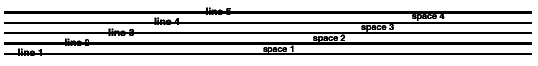
\includegraphics[width=3in,height=3.5in,clip,keepaspectratio]{resources/images/staff_line}
\centering
\caption{Staff Lines}
\end{figure}

\begin{figure}
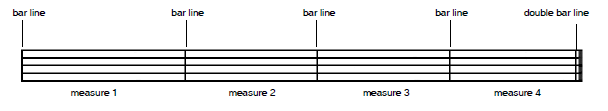
\includegraphics[width=3in,height=3.5in,clip,keepaspectratio]{resources/images/measure_lines}
\centering
\caption{Staff with measures marked}
\end{figure}


\begin{figure}
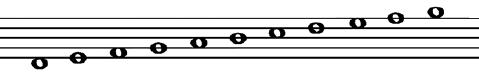
\includegraphics[width=3in,height=3.5in,clip,keepaspectratio]{resources/images/notes}
\centering
\caption{Space notes and line notes on the staff}
\end{figure}

\begin{figure}
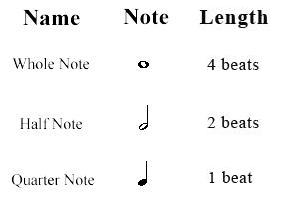
\includegraphics[width=1.5in,height=1.5in,clip,keepaspectratio]{resources/images/note_types}
\centering
\caption{Space notes and line notes on the staff}
\end{figure}

\subsubsection{Notes}`
Depending on the position of the notes on the stafflines, there are 2 types of notes. 
\begin{itemize}
  \item \textbf{Space Notes}: A space note is a note whose note head fits within a space on the staff.
  \item \textbf{Line Notes}: Any note with a line through it.
\end{itemize}
These variations in writing the notes on the staff lines are used to differentiate the pitch of the
notes. Pitch is the highness or lowness of a note. It is determined by the frequency of the waves
producing it. See Fig. 3.

\subsubsection{Note lengths}
There are different types of notes depending on the number of beats. In this
project, the recognition and the playback have been implemented for whole note, half note
and quarter note. Note lengths and symbols are as shown in the Fig. 4.

\subsubsection{Note head and stem}
Note head is the round part. The position of the note head gives the
pitch. The stem is the part that sticks up or down from the head.Whole notes do not have
stems. Quarter notes and half notes have stems. Refer to Fig. 5 .The stem can go either up or down. When a note is on the third line of the staff or below, stems grow up from the right side of the staff head. Refer to Fig. 6 .If the notes are on the third line or below, the stems go down on the left side. Refer to Fig. 7.

\begin{figure}
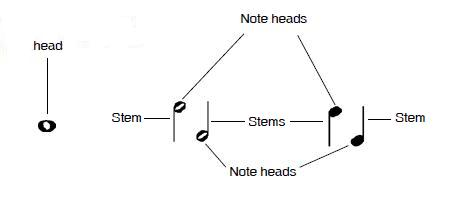
\includegraphics[width=3in,height=3.5in,clip,keepaspectratio]{resources/images/note_head_stem}
\centering
\caption{Note head and stem}
\end{figure}

\begin{figure}
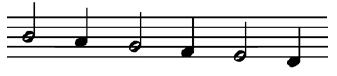
\includegraphics[width=3in,height=3.5in,clip,keepaspectratio]{resources/images/stemp_up_notes}
\centering
\caption{Notes with stem up}
\end{figure}

\begin{figure}
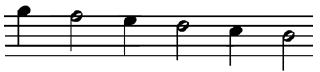
\includegraphics[width=3in,height=3.5in,clip,keepaspectratio]{resources/images/stemp_down_notes}
\centering
\caption{Notes with stem down}
\end{figure}

\begin{figure}
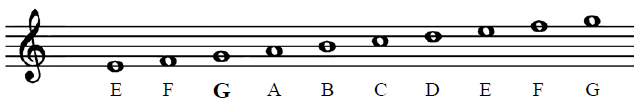
\includegraphics[width=3in,height=3.5in,clip,keepaspectratio]{resources/images/treble_cleff}
\centering
\caption{Treble clef with note names}
\end{figure}

\begin{figure}
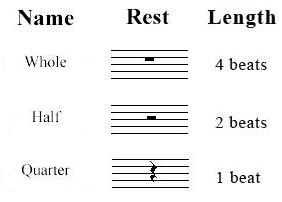
\includegraphics[width=1.5in,height=3.5in,clip,keepaspectratio]{resources/images/rest}
\centering
\caption{Types of rests}
\end{figure}

\begin{figure}
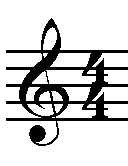
\includegraphics[width=1.0in,height=1.0in,clip,keepaspectratio]{resources/images/time_signature_4_4}
\centering
\caption{4/4 time signature}
\end{figure}

\begin{figure}
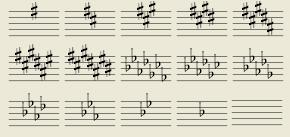
\includegraphics[width=3.0in,height=2.0in,clip,keepaspectratio]{resources/images/key_signatures}
\centering
\caption{Key signatures}
\end{figure}

\subsubsection{Note Names}
The music alphabet uses A,B,C,D,E,F and G. The notes are named alphabetically when the notes are written one after the other.

\subsubsection{Treble Clef}
A clef is a symbol used at the beginning of a musical staff to tell the reader which letter name
goes with which line or space. The treble clef is the most common. It is also called as G clef as it
shows where the note G is on the staff. The inner loop of the treble clef circles the second line of
staff. Refer to Fig. 8.

\subsubsection{Rests}
Rests define the silence in music. Depending on the duration of rest there are different types of
rests. They are shown in Fig. 9.

\subsubsection{Time Signature}
It appears at the beginning of every piece of music score. It gives the information of how many
beats are in each measure.
For example a 4/4 time signature is used to indicate that there will be 4 beats in each measure. Refer to Fig. 10.

\subsubsection{Key Signatures}
The key signature fits between the clef and the time signature. A key signature tells which notes
have flats or sharps for an entire piece of music. Key signature are produced from the combinations
of flats and sharps. There are 15 key signatures common to all the instruments and are shown in
Fig. 11. The symbols of the music sheet described in this chapter are the symbols that have been recognized by the implemented Optical Character Recognition for Music notes and playback system.



% needed in second column of first page if using \IEEEpubid
%\IEEEpubidadjcol

% An example of a floating figure using the graphicx package.
% Note that \label must occur AFTER (or within) \caption.
% For figures, \caption should occur after the \includegraphics.
% Note that IEEEtran v1.7 and later has special internal code that
% is designed to preserve the operation of \label within \caption
% even when the captionsoff option is in effect. However, because
% of issues like this, it may be the safest practice to put all your
% \label just after \caption rather than within \caption{}.
%
% Reminder: the "draftcls" or "draftclsnofoot", not "draft", class
% option should be used if it is desired that the figures are to be
% displayed while in draft mode.
%
%\begin{figure}[!t]
%\centering
%\includegraphics[width=2.5in]{myfigure}
% where an .eps filename suffix will be assumed under latex, 
% and a .pdf suffix will be assumed for pdflatex; or what has been declared
% via \DeclareGraphicsExtensions.
%\caption{Simulation Results}
%\label{fig_sim}
%\end{figure}

% Note that IEEE typically puts floats only at the top, even when this
% results in a large percentage of a column being occupied by floats.


% An example of a double column floating figure using two subfigures.
% (The subfig.sty package must be loaded for this to work.)
% The subfigure \label commands are set within each subfloat command, the
% \label for the overall figure must come after \caption.
% \hfil must be used as a separator to get equal spacing.
% The subfigure.sty package works much the same way, except \subfigure is
% used instead of \subfloat.
%
%\begin{figure*}[!t]
%\centerline{\subfloat[Case I]\includegraphics[width=2.5in]{subfigcase1}%
%\label{fig_first_case}}
%\hfil
%\subfloat[Case II]{\includegraphics[width=2.5in]{subfigcase2}%
%\label{fig_second_case}}}
%\caption{Simulation results}
%\label{fig_sim}
%\end{figure*}
%
% Note that often IEEE papers with subfigures do not employ subfigure
% captions (using the optional argument to \subfloat), but instead will
% reference/describe all of them (a), (b), etc., within the main caption.


% An example of a floating table. Note that, for IEEE style tables, the 
% \caption command should come BEFORE the table. Table text will default to
% \footnotesize as IEEE normally uses this smaller font for tables.
% The \label must come after \caption as always.
%
%\begin{table}[!t]
%% increase table row spacing, adjust to taste
%\renewcommand{\arraystretch}{1.3}
% if using array.sty, it might be a good idea to tweak the value of
% \extrarowheight as needed to properly center the text within the cells
%\caption{An Example of a Table}
%\label{table_example}
%\centering
%% Some packages, such as MDW tools, offer better commands for making tables
%% than the plain LaTeX2e tabular which is used here.
%\begin{tabular}{|c||c|}
%\hline
%One & Two\\
%\hline
%Three & Four\\
%\hline
%\end{tabular}
%\end{table}


% Note that IEEE does not put floats in the very first column - or typically
% anywhere on the first page for that matter. Also, in-text middle ("here")
% positioning is not used. Most IEEE journals use top floats exclusively.
% Note that, LaTeX2e, unlike IEEE journals, places footnotes above bottom
% floats. This can be corrected via the \fnbelowfloat command of the
% stfloats package.

\section{MusicXML}
MusicXML (Music Extensive Markup Language) is a digital sheet music interchange and distribution format. The goal is to create a universal format for common Western music notation, similar to the role that the MP3 format serves for recorded music.\par
The musical information is designed to be usable by notation programs, sequencers and other performance programs, music education
programs and music databases. It is designed from the ground up for sharing sheet music files between applications and for archiving sheet music files for use in the future. MusicXML files are
readable and usable by a wide range of music notation applications. MusicXML complements the
native file formats used by several musical score writing programs, which are designed for rapid
and interactive use. MusicXML
files are the standard for sharing interactive sheet music. Using MusicXML, users can create music
in one program and share the results – back and forth – with people using other programs. \par
MusicXML was based primarily on two academic music formats:
\begin{itemize}
  \item The MuseData format, developed by Walter Hewlett at the Center for Computer Assisted Research in the Humanities (CCARH), located at Stanford University .
  \item The Humdrum format, developed by David Huron, based at Ohio State University.
\end{itemize}
MusicXML has two different top-level Document Type Defitions (DTDs), each with its own
root element. If the partwise DTD is used, the root element is  \textless score-partwise\textgreater . The musical part
is primary, and measures are contained within each part. If the timewise DTD is used, the root
element is \textless score-timewise\textgreater. The measure is primary, and musical parts are contained within each
measure. The MusicXML XML Schema Definition (XSD) includes both of the top-level document
elements in a single XSD file.Having two different structures does not work well if there is no
automatic way to switch between them. MusicXML provides two EXtensible Stylesheet Language
Transformations (XSLT) stylesheets to convert back and forth between the two document types. \par
Score header contains some basic metadata about a musical score, such as the title and composer.
It also contains the part-list, which lists all the parts or instruments in a musical score.
MusicXML music data contains two main types of elements. One set of elements is used primarily to represent how a piece of music should sound. These are the elements that are used when
creating a MIDI file from MusicXML. The other set is used primarily to represent how a piece of
music should look.These elements are used when creating a MuseScore file from MusicXML. The terminology used in XML are as follows.

\subsubsection{Tag}
 A markup construct that begin with ``\textless" and ends with `` \textgreater ". There are three types of tags namely start tags, end tags and empty element tag.

\subsubsection{Element}
An XML element is the central building block of any XML document. It is a logical document component which begins with a start tag and ends with an end tag.

\subsubsection{Root element}
The root element is the first named tag of every XML file and is a container for all other elements.

\subsubsection{Parent element}
An XML element that contains another element.

\subsubsection{Child element}
 An XML element that is contained within a parent element. A child element sits inside of the parent and further itemizes the tags within the file.
 
 \subsubsection{Attribute}
  A markup construct consisting of a name \& value pair that exists within a start tag
or element tag.

\subsubsection{Data String}
 A data string is the information that the viewer can see. For example, a description of an inventory item would be a data string. Data strings sit between the opening and
closing tags of element.

\subsubsection{XML declaration}
The declaration statement gives the browser information to recognize
the language and syntax of the file. Without a declaration statement, the Internet processor
is unable to compute the code. This is the first line of any XML document and defines the
language, version, specifies encoding and declares the standalone status of the file. Only
the language definition and version are required for a declaration statement. Encoding and
standalone are optional attributes.

\section{Software Requirements}
 The input image acquired has to be subjected to various processing operations for recognising the characters in the music score sheet. Thus, the platform used for the implementation  should support
image processing operations. Matlab has extensive support for image processing operations through “Image Processing Toolbox". Matlab also has “Data and File Management Toolbox” which can be used to read, write and generate XML files. MusicXML being one of the types of XML file, the toolbox will be able to handle it's basic operations also. Hence Matlab becomes a good choice for implementation. Matlab version R2014a - 8.3.0.532 has been used for the implementation of the algorithm. For reading MusicXML files “MuseScore” can be used. MuseScore is a free and opensource score writer software with rich features.

\section{Implementation}
This section presents the steps involved in converting the captured image of a score sheet into MusicXML file. Fig. 12 provides the graphical representation of sequence of operations involved in the conversion of image of a score sheet to MusicXML file.


\subsection{Image Acquisition}
 The music score sheet image is acquired from MuseScore software. The file format used is ``png". A sample image of score sheet is shown in Fig. 13.
 
 
 \subsection{Image Preprocessing}
  The image acquired will be in rgb format and is converted into grey scale image. The purpose of converting an RGB image into gray scale is due to the fact that it eliminates the hue and saturation information, as they contribute very less for the total appearance of the image and retains the needed luminance (intensity).  The main advantages of image preprocessing are it helps in reducing the noise in images, Variations in illumination and viewing geometry between images (for optical sensors) can be corrected by image pre-processing techniques and helps to convert the image into a form that is more suitable for further
operations like morphological operations and feature extraction.

\subsection{Image Segmentation}
Image segmentation is the process of partitioning an image into parts or regions. This division into parts is often based on the characteristics of the pixels in the image. Thresholding method of segmenting method is used here to convert a grey scale image into binary image. This transformation is important because the morphological operations like dilation, erosion, etc. can be done efficiently on a binary image. Examples of a segmented image and a non-segmented image are shown in Fig. 14 and Fig. 15. Fig. 15 contains pixel values in the gray scale and each pixel can take any value out of the available 256 gray scale levels.

\begin{figure}
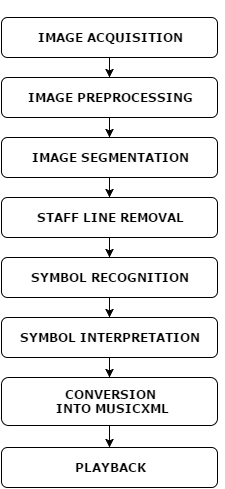
\includegraphics[width=3in,height=3.5in,clip,keepaspectratio]{resources/flowchart/flowchart}
\centering
\caption{Sequence of operations involved in the conversion of image of a score sheet to MusicXML file}
\end{figure}

\begin{figure}
\includegraphics[width=3in,height=3.5in,clip,keepaspectratio]{resources/implementation/good_tone}
\centering
\caption{Music Score sheet image given as input}
\end{figure}

\begin{figure}
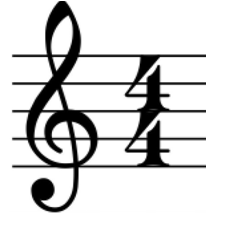
\includegraphics[width=1in,height=1.5in,clip,keepaspectratio]{resources/implementation/non_segmented_image}
\centering
\caption{A non segmented image}
\end{figure}

\begin{figure}
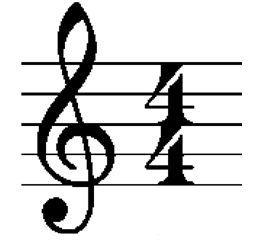
\includegraphics[width=1.0in,height=1.5in,clip,keepaspectratio]{resources/implementation/segmented_image}
\centering
\caption{A segmented image}
\end{figure}

\subsection{Morphological Image processing}
Morphological image processing is a collection of non-linear operations related to the shape or morphology of features in an image. Morphological operations rely only on the relative ordering of
pixel values, not on their numerical values and therefore are especially suited to the processing of binary images. Morphological techniques typically probe an image with a small template known as a Structuring Element (SE). The SE is very small compared to the image size. They are usually made up of
ones and zeroes. The SEs usually have odd orders like 3x3, 5x5, 7x7 etc. because, while performing any morphological operations, the center pixel of the SE is placed on each and every pixel of the
image and the operation is thus performed. The SE is positioned at all possible locations in the image and it is compared with the corresponding neighborhood pixels. By marking the locations
where SE fits or hits the image, information about the structure of the image can be obtained. The SE ``fits” image if for each of its pixels that is set to 1(foreground), the corresponding image pixel
is also set to 1.\par Dilation and erosion are morphological image processing techniques which are extensively used in staff line removal.

\subsection{Staff Line Removal}
 Removing staff lines is important, because
in the score sheet essentially the same symbol will be placed on different staff lines. Without this step, the same symbol will be treated as different when they are on different staff lines. For removal of staff lines morphological image processing techniques such as dilation and erosion are used. The image is subjected to dilation two times which is then followed by erosion.

\subsubsection{Dilation}
The dilation of an image f by a structuring element s (denoted by $ f \oplus s $)
produces a new binary image 
\[g = f \oplus s \] 
with ones in all locations (x,y) of a structuring element’s origin at which that structuring element s fits the the input image f, i.e. g(x,y) = 1 if s fits f and 0 otherwise, repeating f, i.e. g(x,y) = 1 if s hits f and 0 otherwise, repeating. \par
The holes enclosed by a single region and gaps between different regions become smaller, and
small intrusions into boundaries of a region are filled in. Fig. 16 shows the effects of dilation on an input image.

\subsubsection{Erosion}
The erosion of a binary image f by a structuring element s (denoted by $ f \ominus s $)
produces a new binary image
\[g = f \ominus s \]
with ones in all locations (x,y) of a structuring element's origin at which that
structuring element s fits the input image f, i.e. g(x,y) = 1 is s fits f and 0 otherwise, repeating for
all pixel coordinates (x,y). \par
Erosion with small square structuring elements shrinks an image by stripping away a layer of
pixels from both the inner and outer boundaries of regions. The holes and gaps between different
regions become larger and small details are eliminated.\par
Larger structuring elements have a more pronounced effect, the result of erosion with a large
structuring element being similar to the result obtained by iterated erosion using a smaller structuring element of the same shape. If s1 and s2 are a pair of structuring elements identical in shape,
with s2 twice the size of s1, then
%\[ f \ominus s2 \thickapprox (f \ominus s1) \ominus s1 \]
Erosion removes small-scale details from a binary image but simultaneously reduces the size of regions of interest, too. By subtracting the eroded image from the original image, boundaries of each region can be found:
\[ b = f - (f \ominus s) \]
where f is an image of the regions, s is structuring element, and b is an image of the region boundaries. Fig. 17 shows the effects of erosion on an input image.

\begin{figure}
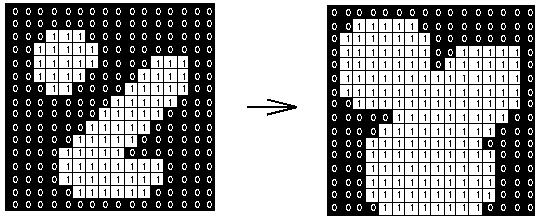
\includegraphics[width=3.0in,height=3.5in,clip,keepaspectratio]{resources/implementation/dilation}
\centering
\caption{Image before and after dilation}
\end{figure}

\begin{figure}
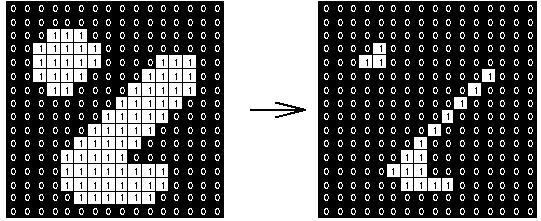
\includegraphics[width=3.0in,height=3.5in,clip,keepaspectratio]{resources/implementation/erosion}
\centering
\caption{Image before and after erosion}
\end{figure}

\subsection{Symbol Recognition}
The symbol recognition is the critical and most important step OCR systems. This step determines the overall performance. Along with the symbol recognition, vertical translation has to be determined to get the output. To recognize the symbols, template matching is used. A template
is a small image (sub-image), the goal is to find occurrences of this template in a larger image. Template matching techniques compare portions of images against one another. Sample images are used to recognize similar objects in source image.\par
Template matching has been a classical approach to the problems of locating and recognizing of an object in an image. Among several matching methods, Normalized Cross Correlation and Square root of Sum of Square Differences have been used as the measure for similarity. Moreover, many other template matching techniques, such as Sum of Absolute Differences (SAD) and Sequential Similarity Detection Algorithm (SSDA) have been adopted in many applications for pattern recognition. In the project Normalized Cross Correlation technique is used for template matching. \par
Correlation is a measure of the degree to which two variables agree, not necessary in actual value but in general behavior. The two variables are the corresponding pixel values in two images, template and source. The cross-correlation of two real continuous functions x(t) and y(t) , is defined by
\[ \phi _{xy} (t) = \int x(t - \tau  )y(\tau)d \tau \]
In comparison to convolution
\[ x(t)*y(t) = \int _{- \infty }^{ \infty } x( \tau - t)*y(\tau)d \tau \]
It can be seen that the only difference is that for the cross correlation, one of the two functions is not reversed.
\[ \phi _{xy} (t) = x(-t)*y(t) \]
Since the operation of time reversal is the same as taking the complex conjugate in the frequency domain.
\[ \phi_{xy} = FT[\phi|xy(t)] = X(f)*Y(f) \]
In the discrete domain, the correlation of two real time series $x_i$, i = 0, 1, . . . , M-1 and $y_j$, j = 0,1, . . . , N-1 is by analogy to equation (1) given by
\[ \phi _{xy, k} = \sum_{j = max(0,k)}^{min(M-1+k, N-1)} x_{j-k} + y_{j} \]
where k = -[M+1],0,(N-1)

\subsection{Normalized Cross Correlation}
The normalized correlation for two time series can be defined as
\[ \phi' _{xy}(t) = \frac{ \phi _{xy}(t) }{ \sqrt{ \phi _{xx}(0)\phi _{yy}(0) } } \]

The normalized quantity will vary between -1 and 1. A value of 1 indicates that at the alignment, the two time series have the exact shape (the amplitudes may be different) while a value -1 indicates that they have the same shape except that they have the opposite signs. A value of 0 shows that they are completely uncorrelated. In practice when one applies this normalization to real discrete signals, one will find that a correlation coefficient greater than about 0.7 or 0.8 indicates a pretty good match. \par

The main advantage of the normalized cross correlation over the ordinary cross correlation is that it is less sensitive to linear changes in the amplitude of illumination in the two compared images. Furthermore, the Normalized Cross Correlation is confined in the range between -1 and 1. The setting of detection threshold value is much simpler than the cross correlation. There are several set of templates which are used to determine the symbols using the normalized
cross correlation method. The database of symbols includes flat, sharp, rests, half note, whole note and quarter note as shown in Fig. 18 to Fig. 22.

\subsubsection{Vertical Translation}
Vertical Translation of a symbol is used to denote its pitch. It is also a crucial parameter in determining the actual symbol. Any error in this step will distort music. Hence it is one part of the recognition where error is intolerable. The position of staff lines in the score sheet is fixed. This principle is useful in finding out the vertical translation. After the normalized cross correlation, the (x,y) coordinate value of the center pixel will be available. Comparing this with the standard value, the vertical translation can be easily obtained. Combining both the symbol and its vertical translation the perfect output is obtained. After this step finally the symbols will be ready for Music
XML conversion and playback.

\begin{figure}
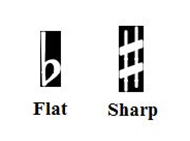
\includegraphics[width=1.5in,height=3.5in,clip,keepaspectratio]{resources/implementation/template_flat_sharp}
\centering
\caption{Templates of sharp and flat symbols}
\end{figure}

\begin{figure}
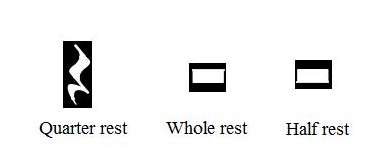
\includegraphics[width=3.5in,height=3.5in,clip,keepaspectratio]{resources/implementation/template_rest}
\centering
\caption{Templates of rests}
\end{figure}

\begin{figure}
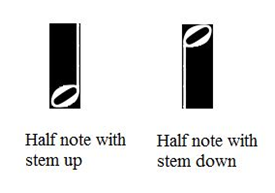
\includegraphics[width=1.5in,height=1.5in,clip,keepaspectratio]{resources/implementation/template_half_note}
\centering
\caption{Templates of half notes}
\end{figure}

\begin{figure}
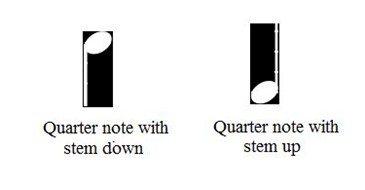
\includegraphics[width=2.5in,height=1.5in,clip,keepaspectratio]{resources/implementation/template_quarter_note}
\centering
\caption{Template of quarter notes}
\end{figure}

\begin{figure}
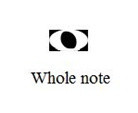
\includegraphics[width=1.5in,height=1.5in,clip,keepaspectratio]{resources/implementation/template_whole_note}
\centering
\caption{Template of whole note}
\end{figure}

\subsection{Symbol Interpretation}
The recognized symbol needs to be interpreted to complete the recognition part. The interpretation part mainly depends on the clef that is used by the music instrument and also it needs to be combined with the vertical translation value to get the final result. When the input is normalized cross correlated with the template, the symbols corresponding to the template will be recognized. After
this step the vertical translation is determined by using the bottom most staff line as a reference. But after this step the output that is produced will have similar symbols next to each other, hence there is a need to put it all together.	



\subsection{Conversion to MusicXML}
For converting the recognized symbols into xml file, the symbols are arranged according to their (x,y) coordinate values. A structure consisting of (x,y) coordinates, staff number, duration, stem, octave, step, voice and alter is created. The structure will be converted into table. The table is sorted and the XML file is generated. The structure for a half note with stem down is shown in Fig. 23. Similarly the structure parameters vary for different notes. The output xml file defines each and every symbol present on the input music score sheet. This file can be played using MuseScore to generate the musical tone. 
The XML file generated consists of the following
\subsubsection{Declaration}

This is the XML declaration required of all XML documents. It specifies that the characters are
written in the Unicode encoding "UTF-8". This is the version of Unicode that has ASCII as a subset.
Setting the value of standalone to "no" means that document is defined with an external definition
in another file.\newline
\textit{ \textless $? xml version=``1.0" encoding=``UTF_8" standalone=``no"? $ \textgreater }

\subsubsection{Root element type}
The \textless score-partwise\textgreater element is made up of parts, where each
part is made up of measures.\newline
\textit{ \textless$score-partwise \enspace version = ``3.0"$\textgreater }  

\subsubsection{ Part id}
The id attribute refers to an id attribute for a score-part in the header. \newline
\textit{ \textless $part id=``P1" $ \textgreater } 

\subsubsection{ Measure number}
Indicates the start of the first measure in the first part.\newline
\textit{ \textless $measure number=``1" $ \textgreater } 

\subsubsection{Attributes}
The attributes element contains key information needed to interpret the notes and musical data
that follow in this part.Attributes contain the following:
\textit{ \textless  attributes \textgreater } 

\subsubsection{ Staves}
The staves element indicates the number of staves in a musical part.

\subsubsection{Clef}
The clef element is used to indicate the clef for the staff. It is used for specifying the clef’s sign
and its line.The treble clef definition indicates that the second line from the bottom of the staff is a G.

\subsubsection{Number}
The number attribute indicates the staff number if the part has more than one staff.

\subsubsection{Stem}
Stem direction is represented with the stem element, whose value can be up, down or none.

\begin{figure}
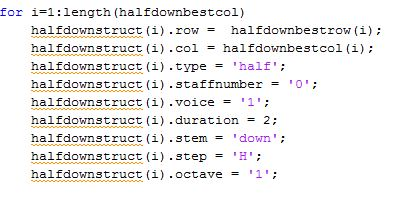
\includegraphics[width=3.5in,height=5.0in,clip,keepaspectratio]{resources/implementation/symbol_interpretation}
\centering
\caption{Structure for half note with stem down}
\end{figure}

\begin{figure}
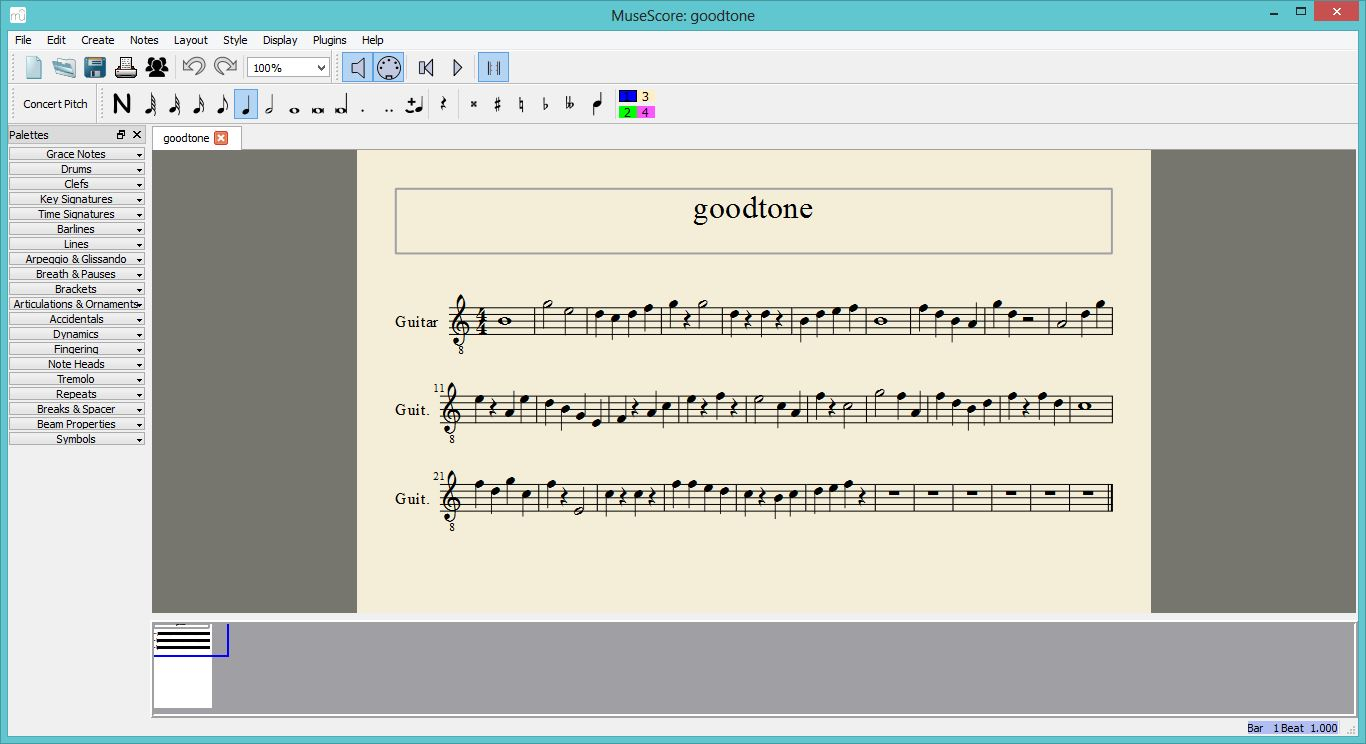
\includegraphics[width=3.5in,height=5.0in,clip,keepaspectratio]{resources/implementation/playback}
\centering
\caption{MuseScore interface}
\end{figure}	

\subsection{Playback}
The playback feature is supported by using MuseScore software. The recognized symbols in
the MusicXML format is imported to MuseScore and played. The recognized score can be seen
in MuseScore and can be compared with the input score sheet for any errors. There are many
features in MuseScore like tempo adjustment, equalizer, mixer and synthesizer for advanced play
back options. The MuseScore interface is as shown in Fig. 24.

\section{Results}
In the section the resulting image from the various stages of OCR is documented.  A sample input image containing the musical notes is taken as input and is shown in Fig. 25. The image consists of various combinations of music symbols such as notes, rests, clefs and time signature. The image is in “.png” format and the file size is 44Kb. The sample input consists of three sets of staff lines.In the next step, staff lines from the image is removed. The output is shown in Fig. 26. Here, it can be observed that the image is complemented and the main reason for this is that the templates
are in the complemented form. In the Fig. 26, even though staff lines are removed, the whole rests and half rests are not damaged. Further, the notes are not distorted. This is the main advantage of using structuring element method for staff line removal. Different images used as templates for the project are as shown in Fig. 18 to Fig. 22. The musical notes are recognized using template matching technique. \par
\begin{figure}
\includegraphics[width=3.5in,height=5.0in,clip,keepaspectratio]{resources/results/good_tone}
\centering
\caption{Input image}
\end{figure}

\begin{figure}
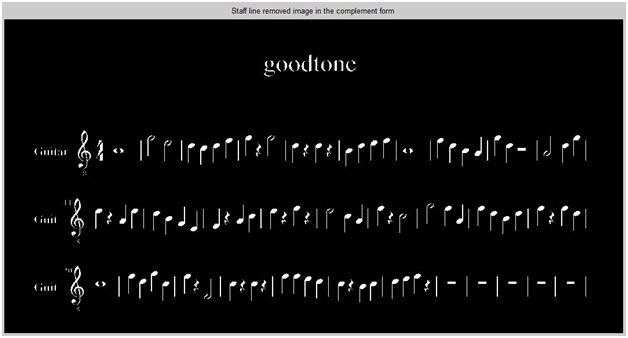
\includegraphics[width=3.5in,height=5.0in,clip,keepaspectratio]{resources/results/good_tone_staff_removed}
\centering
\caption{Staff line removed image}
\end{figure}

\begin{figure}
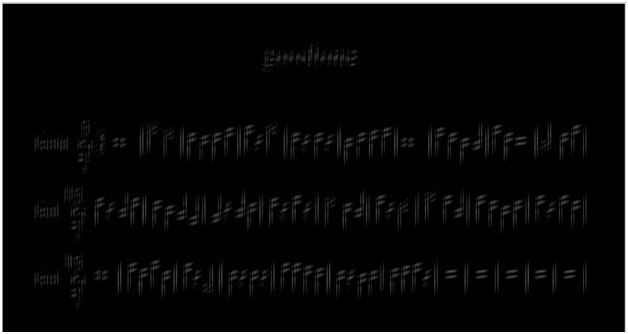
\includegraphics[width=3.5in,height=5.0in,clip,keepaspectratio]{resources/results/normalized_cross_correlation}
\centering
\caption{Normalized cross correlated output of the input image with the ‘Sharp’ template}
\end{figure}

\begin{figure}
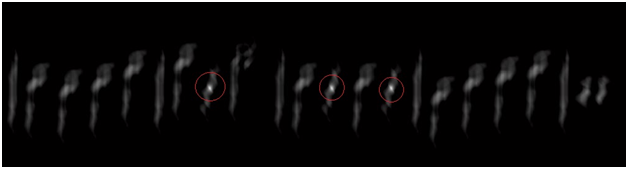
\includegraphics[width=3.5in,height=5.0in,clip,keepaspectratio]{resources/results/matched_symbols}
\centering
\caption{The center pixels with maximum value after cross correlation}
\end{figure}

\begin{figure}
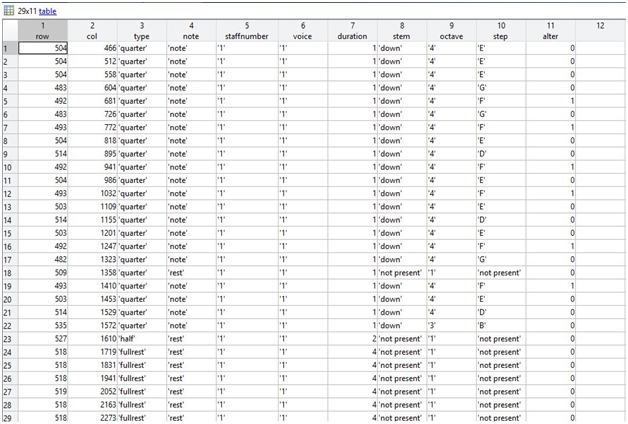
\includegraphics[width=3.5in,height=5.0in,clip,keepaspectratio]{resources/results/symbol_table}
\centering
\caption{Symbol table for image}
\end{figure}

\begin{figure}
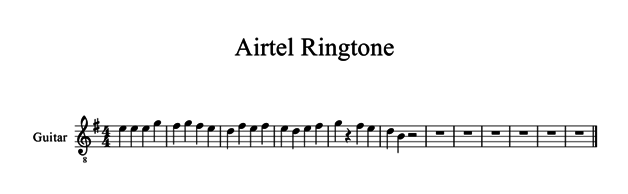
\includegraphics[width=3.5in,height=5.0in,clip,keepaspectratio]{resources/results/airtel}
\centering
\caption{Symbol table for image}
\end{figure}

\begin{figure}
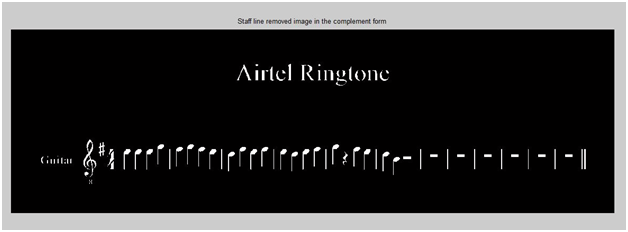
\includegraphics[width=3.5in,height=5.0in,clip,keepaspectratio]{resources/results/airtel_staff_line_removed}
\centering
\caption{Symbol table for image}
\end{figure}

After staff line removal, the image is cross correlated with the template images and normalized. The output is as shown in Fig. 27. In this method, only the symbols same as the template will have the maximum value of cross correlated coefficients as shown in Fig. 28 and all other symbols will have minimum value of cross correlated coefficients. This method can identify all similar symbols in single iteration. Same step is repeated with all the templates to recognize all the symbols. \par
After the normalized cross correlation, the symbol is identified and corresponding XML symbols will be generated. This xml file can be imported to MuseScore software for playback. Currently the system supports 10 different instruments such as guitar, violin, mandolin, melodica, banjo,koto, kazoo, electric guitar, sitar and mezzo-soprano.For cross verification of the correctness of the symbols, a table consisting of symbol name, its (x,y) coordinates, staff number, duration, stem, octave, step, voice and alter is generated. This step is useful in error rectification if there are any from the system. The symbol table for the small portion of airtel ring tone is as shown in Fig. 29. The score sheet is shown in Fig. 30 and the staff line removed output is shown in Fig 31.



% if have a single appendix:
%\appendix[Proof of the Zonklar Equations]
% or
%\appendix  % for no appendix heading
% do not use \section anymore after \appendix, only \section*
% is possibly needed

% use appendices with more than one appendix
% then use \section to start each appendix
% you must declare a \section before using any
% \subsection or using \label (\appendices by itself
% starts a section numbered zero.)
%

% use section* for acknowledgement
\section*{Acknowledgment}

I would like to thank my team mates for their support and Prof. Nataraj C.R. for his valuable guidance without which the project would not have been possible
% Can use something like this to put references on a page
% by themselves when using endfloat and the captionsoff option.
\ifCLASSOPTIONcaptionsoff
  \newpage
\fi



% trigger a \newpage just before the given reference
% number - used to balance the columns on the last page
% adjust value as needed - may need to be readjusted if
% the document is modified later
%\IEEEtriggeratref{8}
% The "triggered" command can be changed if desired:
%\IEEEtriggercmd{\enlargethispage{-5in}}

% references section

% can use a bibliography generated by BibTeX as a .bbl file
% BibTeX documentation can be easily obtained at:
% http://www.ctan.org/tex-archive/biblio/bibtex/contrib/doc/
% The IEEEtran BibTeX style support page is at:
% http://www.michaelshell.org/tex/ieeetran/bibtex/
%\bibliographystyle{IEEEtran}
% argument is your BibTeX string definitions and bibliography database(s)
%\bibliography{IEEEabrv,../bib/paper}
%
% <OR> manually copy in the resultant .bbl file
% set second argument of \begin to the number of references
% (used to reserve space for the reference number labels box)
\begin{thebibliography}{1}
  
\bibitem{IEEEhowto:bullen}
Andrew H Bullen,``Bringing Sheet Music to Life: My Experiences with OMR". \emph{The code\{4\}lib Journal}, Issue 3, 2008.

\bibitem{IEEEhowto:bainbridgei}
David Bainbridgei and Tim Bell,``The Challenge of Optical Music Recognition". \emph{Computer and Humanities, Kulwer Academic Publishers}, 35(2): 95-121, 2001.

\bibitem{IEEEhowto:bainbridgei}
Donald Byrd,``OMR - Optical Music Recognition Systems". \emph{Computer and Humanities, Kulwer Academic Publishers}, 35: 95–121, 2001.

\bibitem{IEEEhowto:bainbridgei}
Ana Rebelo,Ichiro Fujinaga,Filipe Paszkiewicz ,Andre R. S. Marcal, CarlosGuedes, Jaime S. Cardoso.,``Optical music recognition: state-of-the-art and open issues". \emph{Springer}, 2012.

\bibitem{IEEEhowto:capela}
A. Rebelo,G. Capela, Jaime S. Cardoso,``Optical recognition of music symbols - A comparative study", \emph{Springer-Verlag} 2009.

\bibitem{IEEEhowto:raphael}
Christopher Raphael and Jingya Wang,``New Approaches to optical music recognition", in \emph{12th International Society for Music Information Retrieval Conference} 2011.

\bibitem{IEEEhowto:Novotn´y}
Jiˇr´ı Novotn´y and Jaroslav Pokorn´y,``Introduction to Optical Music Recognition:Overview and Practical Challenges", in \emph{CEUR Workshop Proceedings, pp. 65-76, Vol-1343 } 2015.

\bibitem{IEEEhowto:jiang}
Christopher Raphael and Yucong Jiang,``Instrument identification in optical music recognition", in \emph{16th International Society for Music Information Retrieval Conference} 2015.

\bibitem{IEEEhowto:harnum}
Jonathan Harnum,``Basic Music Theory",\emph{Sol-UT Press} 2001.

\bibitem{IEEEhowto:gonzalez}
R.C. Gonzalez, R.E. Woods,``Digital Image Processing second edition",\emph{Prentice Hall} 2002.


\end{thebibliography}

% biography section
% 
% If you have an EPS/PDF photo (graphicx package needed) extra braces are
% needed around the contents of the optional argument to biography to prevent
% the LaTeX parser from getting confused when it sees the complicated
% \includegraphics command within an optional argument. (You could create
% your own custom macro containing the \includegraphics command to make things
% simpler here.)
%\begin{biography}[{\includegraphics[width=1in,height=1.25in,clip,keepaspectratio]{mshell}}]{Michael Shell}
% or if you just want to reserve a space for a photo:


% You can push biographies down or up by placing
% a \vfill before or after them. The appropriate
% use of \vfill depends on what kind of text is
% on the last page and whether or not the columns
% are being equalized.

%\vfill

% Can be used to pull up biographies so that the bottom of the last one
% is flush with the other column.
%\enlargethispage{-5in}



% that's all folks
\end{document}

